%SIGMETRICS
%\documentclass{sig-alternate}

%USENIX
\documentclass[letterpaper,twocolumn,10pt]{article}
\usepackage{usenix,epsfig,endnotes}

\usepackage[noend]{algpseudocode}
\usepackage{paralist,algorithm}
\usepackage{booktabs}
\usepackage{subcaption}
\usepackage{multirow}
\usepackage{float}
\usepackage{graphicx}
\usepackage{pgfplots}
\usepackage{amssymb}
\usepackage{epstopdf}
\usepackage{tikz}
\usepackage{tkz-tab}

%\usepackage{epsfig}
%\epstopdfsetup{outdir=./}
%\usepackage[showframe=true]{geometry}
\usepackage{enumitem}

%ACM
% ---- TR: remove copyright box -------------
% \usepackage{etoolbox}
% \makeatletter
% \patchcmd{\maketitle}{\@copyrightspace}{}{}{}
% \makeatother
% ---- TR: remove copyright box -------------


\begin{document}

%USENIX
\date{}

\title{\Large \bf Parikshan: Debugging Production Systems in Isolation}

\iffalse
\author{
{\rm Nipun Arora$^\dagger$, Franjo Ivan\v{c}i\'{c}}\\$^*$, Gail Kaiser$^\ddagger$}\\
$^\dagger$NEC Laboratories America \hspace{1.4cm}   $^\*$Google NYC \hspace{1.4cm}  $^\ddagger$Columbia University\\
nipun@nec-labs.com \hspace{4pt} ivancic@google.com \hspace{4pt} kaiser@cs.columbia.edu \\
}
\fi

%\iffalse
\author{
{\rm Nipun Arora}\\
       NEC Research Labs\\
       Princeton, NJ, USA\\
       nipun@nec-labs.com
\and
{\rm Franjo Ivan\v{c}i\'{c}}\\
       Google\\
       New York, NY, USA\\
       ivancic@google.com
\and
{\rm Gail Kaiser}\\
       Columbia University\\
       New York, NY, USA\\
       kaiser@cs.columbia.edu
}
%\fi

\maketitle


%SIGMETRICS
\begin{abstract}
\noindent
One of the biggest problems faced by developers debugging large scale systems is replicating the deployed environment to figure out errors. 
Additionally, many modern companies are combining their development and operation management activities (DevOps), which has led to an increased emphasis on fast bug resolution. 
In this work we present \textit{``live-debugging''}, a mechanism which allows debugging a production system (run test-cases, debug, or profile, etc.) on-the-fly. 
%in a sandbox environment cloned from the live running system. 
The paper leverages user-space containers (OpenVZ/LXC) to launch containers cloned and migrated from running instances of an application, thereby launching two containers: \textit{production} (which provides the real output), and \textit{debug-container} (for debugging). 
This \emph{debug-container} provides a sandbox environment for debugging without any perturbation to the execution environment. 
%Our sandboxes provide name-space, and resource management for the processes executing the test/debug cases. 
Customized network-proxy agents replicate or replay network inputs from clients to both the production and debug-container, as well as safely discard all network output from the debug-container. 
The sandboxed debug-container can be run either on the same physical host as the production container, or scaled out on dedicated physical debug servers. 
We used our system, called \texttt{Parikshan}, to do \textit{``live-debugging''} on several real-world bugs, and effectively reduced debugging complexity and time.
%We believe our tool provides a mechanism for practical live-debugging of large scale multi-tier and cloud applications, without requiring any application down-time, and minimal performance impact.

\noindent
\textbf{Tags:} live cloning, network duplication, live debugging
\end{abstract}

%In recent years there has been a lot of work in record-and-replay systems which captures traces from live production systems, and replays them.
%However, most such record-replay systems have a high recording overhead and are still not practical to be used in production environments without paying a penalty in terms of user-experience. 


%SIGMETRICS
% A category with the (minimum) three required fields
%\category{H.4}{Information Systems Applications}{Miscellaneous}
%A category including the fourth, optional field follows...
%\category{D.2.8}{Software Engineering}{Metrics}[complexity measures, performance measures]
%\terms{Theory}
%\keywords{ACM proceedings, \LaTeX, text tagging}

\newcommand{\iprobe}{\texttt{iProbe}}
\newcommand{\parikshan}{\texttt{Parikshan} }

\section{Introduction}
\label{sec:introduction}

Software bugs are \emph{everywhere}.
They often escape extermination efforts in software testing causing frustration to operators, and a loss of business revenue.
\emph{Bug Diagnosis} is the ``art'' of identifying the root-cause and the possible ``fix'' for the failure.
In general the process involves a trial-and-error process in the development environment. 
The debugger uses the input causing the failure and tries to localize the problem in a small part of the application.
He then manually skims through the code in the localized area to correctly identify the problem.
This process can be long and arduous, causing significant loss of revenue.

We believe that by closing the gap between the production and debugging environment, we can provide the developer with a deeper insight of the cause of the bug.
Our previously proposed approach called \livedebugging~\cite{livedebugging}, we have developed a framework which allows debuggers to safely debug applications within the production environment.
This is done by creating a parallel debugging environment, which gets the same input as the normal production system.
This debugging environment provides a powerful tool for the debugger, to freely instrument or modify the application without impacting the performance of the production system.

In this work, we focus on real-time debugging techniques, which can be used on the production environment.
Firstly, we will present an adaptive guided profiling mechanism, which can provide rich profiles in order to localize the bug, while keeping the instrumentation overhead within a preset limit(called budget).
We are inspired by previous approaches in delta debugging~\cite{delta}, and statistical debugging~\cite{statistical, holmes}. 
These approaches use sampled profiles from predetermined instrumentation points, and compare traces, with and without the bug, to localize the problem.
Holmes~\cite{holmes} in particular also includes a feedback loop, which iteratively modifies the instrumentation profiles to gather more relevant traces.
We use a similar technique along with dynamic instrumentation to iteratively change profiles to get a better understanding of the root-cause of the error while debugging the application on-the-fly.
Budgeting the overhead is important so that the instrumentation in the debug environment does not make it lag too far behind the production environment.

Secondly, we will also look at a more proactive approach, where we modify the debug container to not simply trace, but see if a potential fix/optimization solves the problem.
We show how for some performance bugs, we can dynamically patch and verify that the problem is indeed solved.

\section{Overview}
\label{sec:overview}


In recent years several monitoring techniques have been developed to monitor the health of production systems.
For example most modern operating systems have resource monitors~\cite{linuxHealth, windowsHealth, macHealth}, which can be used to track the CPU, memory usage, cache misses, temperature etc. of the physical machine.
These are useful to discover high workloads, or if the machine is stressed because of heavy resource usage.
Similarly, application level monitoring tools are used to report transactions or errors in the application.
Monitoring outputs usually provide the first clue towards resolving an error in the debugging process.
%While useful, these monitoring mechanisms  have a performance trade-off with the amount of instrumentation that can be done.
%Furthermore, the information provided by these logs may not be enough to understand the root-cause of the error.

However all monitoring/instrumentation techniques impose a performance overhead on the applications.
This can adversely impact user-experience, hence real-world production instrumentation is generally kept at very low levels.
\parikshan provides an alternative mechanism where this debugging/instrumentation can be done in parallel on a sandboxed cloned container.
Any instrumentation or monitoring in the debug-container has no performance impact on the production container.
In the context of our system, debuggers can use a variety of ad-hoc approaches to capture the root-cause of an error.
For example a naive approach could be to use trial-and-error instrumentation to find the execution trace for the error.
Alternatively, the user could also do aggressive brute force instrumentation for all function execution, which could help locate the problem.
However, both these approaches can have potentially high overheads, which in turn can lead to a buffer overflow.

In this chapter we introduce a statistical sampling approach which imposes a bounded performance overhead, to ensure maximal live debugging information, without causing a buffer overflow.
%In our search for more systematic approach towards live debugging, we looked towards two possible techniques.
%Firstly, we try to implement an automated budget limited instrumentation approach for capturing application logs.
We are inspired by previous work done in statistical debugging~\cite{cbi}, and delta debugging~\cite{delta} techniques which aim to streamline and automate the process of bug localization.
This is achieved by having predicate profiles from both successful and failing runs of a program and applying statistical techniques to pinpoint the cause of the failure.
The core advantage of statistical debugging is that the sampling frequency of the instrumentation can be decreased to reduce the instrumentation overhead.

One of the key criteria for successful statistical debugging is to have higher instrumentation rates, to make the results more statistically significant. 
There is a clear trade-off between instrumentation vs performance overhead for statistical instrumentation. 
A key advantage of using this with \parikshan is that we can provide live feedback based buffer size and bounded overheads, hence squeezing the maximum advantage out of statistical debugging without impacting the overhead. 
We evaluate the slack available in each request for instrumentation without risking a buffer overflow and getting out of sync of the production container.
Live interactive debugging provided by \parikshan further allows for quick updates to the instrumentation and targeting specific areas of the application code.

%\section{Motivating Scenario}
%\subsection{Motivating Scenario}
\label{sec:motivation}

\begin{figure*}[ht!]
  \begin{center}
%    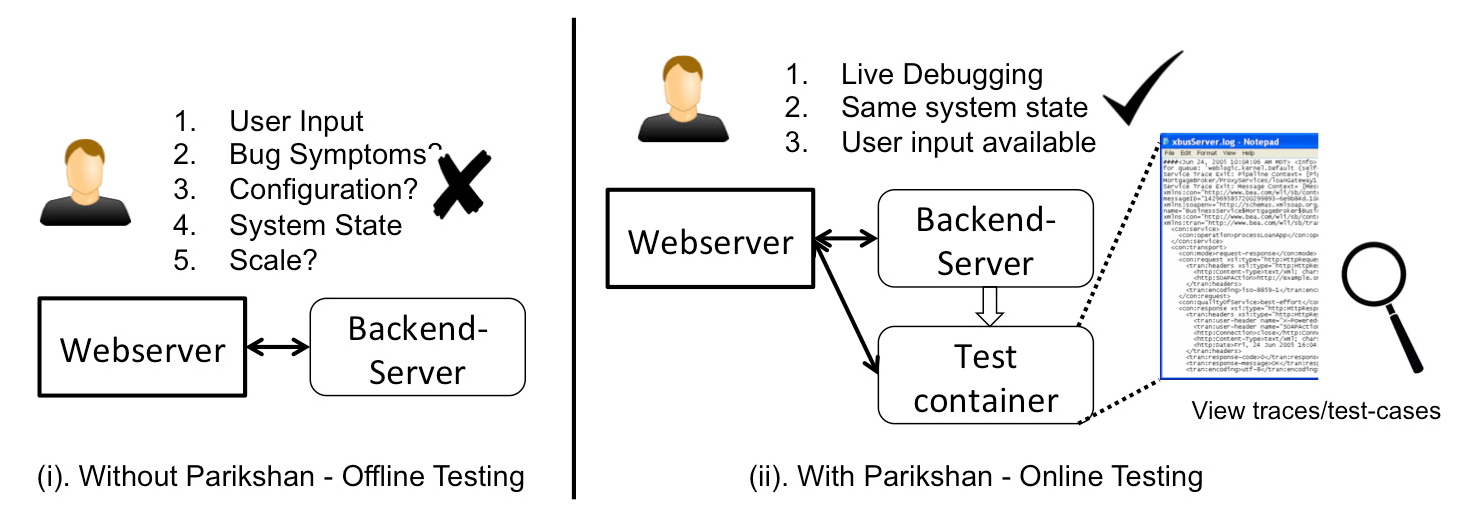
\includegraphics[width=0.7\textwidth]{figs/motivation.eps}
    \includegraphics[width=0.95\textwidth]{figs/workflow3.pdf}
    \caption{Workflow of \parikshan in a live multi-tier production system with several interacting services. When the administrator of the system observes errors in two of it's tiers, he can create a sandboxed clone of these tiers and observe/debug them in a sandbox environment without impacting the production system.}
    \label{fig:motivation}
  \end{center}
\end{figure*}

\noindent
As a motivating scenario, let us take a complex multi-tier service-oriented system (Figure \ref{fig:motivation}), with several interacting services (web-servers, application servers, search and indexing, database etc.). 
The system is maintained by an operator, who can observe the health of the system using light-weight monitoring, which is part of the deployed system.
In the interest of application performance, production system monitoring is usually limited to system resource usage, application usage statistics, transaction logs, and error logs.

At a certain time in the execution of the system, the operator observes unusual memory usage in the glassfish application server, and some error logs being generated in the nginx web-server. 
He surmises, that there is a potential memory leak/allocation problem in the app-server, or a problem in the web-server.
However, with a limited amount of monitoring information, he can only go so far.

\iffalse
user Joe who is an administrator for a multi-tiered system (see Figure \ref{fig:motivation}). 
Much like several administrators, Joe uses light-weight system instrumentation to get a high level statistical/health view of the system.
He observes an unusually high memory usage in the glassfish server for transaction type X, and some anomalous error logs in the associated nginx systems.
Under usual circumstances, the system would have to go down(depending on the severity of the problem), the problem debugged using offline analysis, and the system would be patched once the problem has been diagnosed. 
However often, it is difficult to find out the configuration of the system, and the user input which is causing this problem.
In modern large scale systems some errors may happen only at scale, and would require a large test-cluster to recreate the error.
Furthermore, taking down the glassfish and nginx servers would impact several more services otherwise are running fine. 
\fi

Typically, trouble tickets are generated for such problems, and they are debugged offline.
However using \parikshan, the operator can fork off clones of the nginx and glassfish containers as \textbf{\textit{nginx-debug}} and \textbf{\textit{glassfish-debug}}.
%Our proxy network duplication now sends a copy of the incoming request to the debug containers, while users can continue using nginx and glassfish services. 
Our network duplication mechanisms ensure that the debug containers receive the same inputs as the production containers, and that the production containers continue to provide service without interruption.
This separation of the production and debug environment, allows the operator to use dynamic instrumentation tools to perform deeper diagnosis without fear of additional disruptions due to debugging.
Since the system has been cloned from the original potentially ``buggy'' production container, it will also exhibit the same memory leaks/or logical errors.
Additionally, \parikshan can focus on the ``buggy'' parts of the system, without needing to replicate the entire system in a test-cluster.
This process will greatly reduce the time to bug resolution, and allow real-time bug diagnosis capability.
%Time to bug resolution is usually a very important criteria in any user-facing service oriented application.
%This , while allowing real-time-diagnosis, significantly reduce the time to bug resolution.

% This paragraph needs serious revision - the points have been noted down but they need to be stated clearly in a better manner.
%One of the key advantages of such an online approach is a reduced time to bug resolution. 
%Time to bug resolution is usually a very important criteria in any user-facing service oriented application, as the longer a bug remains the system, the more it is going to hit the user perception/revenue.
%Bearing this in my mind we believe, that online testing will be an important aspect towards modern applications.
%Additionally the usage of redundant computing for testing in A/B testing(see section \ref{sec:related}) approaches is a well accepted paradigm in real-world applications.
%This leads us to believe that using redundant computing will be acceptable for regular testing approaches as well.
%Using \parikshan is also a way to avoid creating a large test-cluster to do debugging. 

\iffalse
\subsection{Motivation Questions?}

To further motivate our testing paradigm we have come up with a set of motivating questions:

%\begin{compactitem}
%\setlength{\itemsep}{1Pt}
%\item[]\textbf{Q1:} Is it important to sandbox test-cases?
%\item[]\textbf{Q2:} Is recreating production environment difficult? 
%\item[]\textbf{Q3:} Is redundant computing available? 
%\item[]\textbf{Q4:} How would executing test-cases in a production server effect user-experience?
%\end{compactitem}

\subsubsection{\textbf{Q1:} Is it persistent testing important?}
\subsubsection{\textbf{Q2:} Is recreating production environment difficult?}
\subsubsection{\textbf{Q3:} Can redundant computing be utilized for testing?}
\subsubsection{\textbf{Q4:} How would executing test-cases in a production server effect user-experience?}
\fi
 \section{Design}
\label{sec:design}

%Each instance of \parikshan can target only one tier at a time.
%However, multiple instances can be orchestrated together to do distributed debug analysis. 
%especially when it's required for integration testing or cross tier results need to be correlated.
%\parikshan can target multiple tiers of a system by cloning the target tiers and stubbing out it's communication with the external environment.
In figure~\ref{fig:workflow}, we show the architecture of \parikshan when applied to a single mid-tier application server.
\parikshan consists of 3 modules: 
\textbf{Clone Manager}: manages ``live cloning'' between the production and the debug containers, 
\textbf{Network Duplicator}: manages network traffic duplication from downstream servers to both the production and debug containers, 
and \textbf{Network Aggregator}: manages network communication from the production and debug containers to upstream servers.
The duplicator, and aggregator can be used to target multiple connected tiers of a system by duplicating traffic at the beginning and end of a workflow.
Furthermore, the aggregator module is not required if the debug-container has no upstream services. 
Network duplication, and aggregation can be used in one or more protocols to partially or completely isolate the debug container, depending on the interacting services and the debugging requirements.
At the end of this section, we also discuss the \textbf{debug window} during which we believe that the debug-container faithfully represents the execution of the production container.
Finally, we discuss \textbf{divergence checking} which allows us to observe if the production and debug containers are still in sync.

%which uses user-space containers OpenVZ~\cite{openvz} and a variant of live migration to implement the cloning.
%To begin with let us look at a simple example of client web-server with a database server as the backend (as shown in Figure \ref{fig:workflow}), where the test harness needs to be applied on the backend.
%As explained earlier basic workflow of our system is to duplicate all network requests to the production backend server and a ``live cloned'' test container.
%Traffic duplication is managed by our proxy network duplicator (see section \ref{sec:proxyDuplicator}), which uses several different strategies to clone user input to our test-container, with minimal impact on the production container.
%Another core aspect of our design is ``live cloning''; this is the process by which a production container (in this case our backend service), can be cloned to create a test-container which has the same file system and process state. 
%Next, we explain each of the modules in detail.
%The architecture can be divided into two parts: (1) A Proxy Network Duplicator, (2) container clone manager
%\begin{itemize} 

\begin{figure}[h]
  \begin{center}
    \includegraphics[width=0.5\textwidth]{figs/arch.png}
    \caption{\parikshan applied to a mid-tier service: It is comprised of: (1) Clone Manager for Live Cloning, (2) Proxy Duplicator to duplicate network traffic, and (3) Proxy Aggregator to replay network traffic to the cloned debug container.}
    \label{fig:workflow}
  \end{center}
\end{figure}


\subsection{Clone Manager} 
\label{sec:CloneManager}

%\subsubsection{How does cloning work?}
%\label{sec:cloning}

%While the focus of our work is not to support container migration, or to make changes to the hypervisor, we need to tweak the way typical hypervisors offer live migration for our purposes.
%Before moving further we wish to clarify that instead of the standard live migration supported by hypervisors, \parikshan requires a cloning functionality. 
%In contrast with live migration, where a container is copied to a target destination, and then the original container is destroyed, the cloning process requires both containers to be actively running, and be still attached to the original network.
%This cloning requires modification in both how compute migration is handled, and especially how the network migration is handled. 

Before describing cloning in our context, let us first review some details about live migration. 
It refers to the process of moving a running virtual machine, guest OS or container from one host node (physical machine) to another, without disconnecting any client or process running within the machine. 
%It is supported by most well known Hypervisors (VMware, VirtualBox, Xen, Qemu, KVM).
% with different amounts of efficiency.
%There are several different mechanisms for migration, some of which require a short suspend time, while others are able to seamlessly transfer without any noticeable down-time by the user.
In general the basic process involves the following steps: 
(1) Firstly, the copy (\textit{rsync}) is initiated by a pre-copy memory migration, where the underlying hypervisor copies all the memory pages from the source to the destination. 
(2) Once the pre-copy phase is finished, the VM is temporarily suspended, and all memory pages including live memory pages are transferred to the target node. 
Once all memory pages have been transferred, the target container is restarted. 
Two rsync runs are needed, so the first one moves most of the data, while the container is still up and running, and the second one moves the changes made during the time period between the first rsync run and the container pause.
The second step can be done in multiple iterations to avoid a long suspend time, incase the memory pages have significantly changed after the first rsync. 
%\footnote{Network migration is managed by the IAAS which publishes the same MAC address for the copied VM. 
%Since the identity of the target container remains the same, the IAAS is able to give it same IP Address, and network traffic is rerouted after the identity is published in the network}.
%To reduce the down-time memory pages are transferred probabiliticly based on priority, and incase a page is not found a network fault is generated which executes a fetch from the original VM.

In contrast with live migration where the original container is destroyed, the ``Live Cloning'' process used in \parikshan requires both containers to be actively running, and be still attached to the original network.
%Instead of Live Migration, in Live Cloning, we do not delete the source container, rather we allow the container to keep executing in both production and test locations.
The challenge here is to manage two containers with the same identities in the network and application domain. 
This is important, as the operating system and the application processes running in it may be configured with the IP address, or other networking operation, which cannot be changed on the fly leading to a crash of the system.
Hence the same network identifier should map to two separate addresses, and have communication with no problems or slowdowns.
\iffalse
Clearly the same IP address or MAX address cannot be kept for both the production and debug-container as that would lead to conflict in the network. 
There are two ways to resolve this: 
(1) Host each container behind their own network namespaces, on the same host machine, and configure packet forwarding to both containers such that the duplicator can communicate to them. 
Network namespaces (see internal mode in Figure~\ref{fig:modesCloning}) 
have been used by several hosting providers, to launch VM's with the 
same private IP address in a shared network domain~\cite{OpenStack}. 
(2) Another approach is to host both containers in different machines with port forwarding setup to forward incoming TCP requests to containers behind a NAT (see external mode in Figure~\ref{fig:modesCloning}). 
This is more scalable and has clear separation of network and compute resources. 
%However, an obvious downside to this approach is that it needs a new VM to be allocated.
%This leads us to two different modes of implementation, which we discuss in the next section.

%As of now, we have implemented the second approach for our proof of concept mostly because of the ease of implementation.
%Further a packet level sniffer or mirror port would keep the same buffer and potentially timeout.
%To allow for some load-balancing and an application aware buffer, we went for a web application level proxy server to duplicate traffic to both containers. 
%Further in this section we explain how we deal with these challenges.

\subsubsection{Basic Design \& Modes}

The Clone Manager itself is just an interface which interacts with an \textit{agent} installed in each container host.
It manages the frequency of cloning/syncing operations, as well as  coordinates setup operations/orchestration etc.
Communication between clone manager, and the agent is done using RPC calls implemented using Apache Thrift~\cite{thrift}.
The agent itself is the driver for live cloning, and performs rsync operations, snapshot, transferring and starting the image.
\fi
%Test and production containers can be allocated in various schemes: we call these schemes \textit{modes}. 
Broadly the clone manager has two modes (see Figure~\ref{fig:modesCloning}) : 

\begin{figure}[t]
  \begin{center}
    \includegraphics[width=0.5\textwidth]{figs/ModesCloning.png}
    \caption{External and Internal Mode for Live Cloning: P1 is the production container, and T1 is the debug container, the Clone Manager interacts with an Agent which has drivers to implement live Cloning}
    \label{fig:modesCloning}
  \end{center}
\end{figure}

\begin{itemize}[leftmargin=*,topsep=0pt,itemsep=-1ex,partopsep=1ex,parsep=1ex]

\item \textit{Internal Mode}: In this mode we allocate the debug-container and  production containers to the same host node. 
This would mean less suspend time, as the production container can be locally cloned (instead of streaming over the network). 
It requires the same amount of resources as the original production container (number of host nodes remain the same), 
hence it could potentially be cost-effective.
On the down-side, co-hosting the debug and production containers could have an adverse effect on the performance of the production container.
This may in turn be observable to the user.
As we can see in Figure~\ref{fig:modesCloning}, the production container P1 and debug container T1 are both hosted within the same physical host, and with the same IP address.
However, their network is encapsulated within different network namespaces to sandbox them.
The duplicator is then able to communicate to both these containers with no networking conflict.

\item \textit{External Mode}: In this mode we provision an extra server as the host of our debug-container (this server can host more than one debug-containers). 
While this mechanism can have a higher overhead in terms of suspend time (3 seconds, dependent on process state), and requires provisioning an extra host-node, the advantage of this mechanism is that once cloned, the VM is totally separate and will not effect the performance of the production-container.

We believe that such a mode will be more beneficial in comparison to the internal mode, as cloning is likely to be transient. 
It is often more important to not effect user experience. 
However, when running in the internal-mode, the test could potentially 
impact the production run due to co-location in the same host 
(resource contention etc.).

As we can see in Figure~\ref{fig:modesCloning}, the production container P1 and debug container T1 are hosted on two different host machines, and are encapsulated behind a NAT~\cite{nat} (network address translator).
Thus, they each have their own IP addresses in an internal network thereby avoiding any 
conflict.\footnote{Another additional mode can be \textit{Scaled Mode}: 
This can be viewed as a variant of the external mode, where we can execute debug analysis in parallel on more than one debug containers which can be used to distribute the instrumentation load to reduce the overhead. 
This is currently out of the scope of this paper, however we aim to show this in a future publication.}

\end{itemize}

%\RestyleAlgo{boxruled}
%\LinesNumbered

%\\ \\
%\noindent \textbf{Implementation}\\

\subsubsection{Algorithm}

%The Clone Manager is responsible for creating a live running ``clone'' of the production container and launch it as the test-container. 
%In our current setup cloning is done for each target production environment in the same physical host machine 
%(we can clone to a different physical host as well, however for optimization purposes we have assumed that they will always be in the same local network).

In our current implementation, we are using OpenVZ~\cite{openvz} as our container engine, and have modified the migration mechanism in vzctl~\cite{vzctl} to make it work for live cloning instead. 
We tested this out on multiple VM's acting as host nodes for OpenVZ containers. 
To make the cloning easier and faster, we used OpenVZ's \textit{ploop} devices~\cite{ploop} to host the containers. 
\textit{Ploop} devices are a variant of disk loopback devices where the entire file system of the container is stored as a single file. 
This allows features such as syncing, moving, snapshots, backups and easy separation of inodes of each container file system.

The algorithm for live cloning is explained below: 
\begin{algorithm}[ht!]
  \caption{Live cloning algorithm using OpenVZ} 
  \label{algCloning}
  \begin{enumerate}[topsep=0pt,itemsep=-1ex,partopsep=1ex,parsep=1ex]
%  \item Safety Checks (Checks that a destination server is available via ssh w/o entering a password, and version checking of OpenVZ running in it) 
  \item Run rsync of source \textit{ploop} file system to the destination server  
  \item Checkpoint and suspend the container 
  \item Run a second rsync of the \textit{ploop} device to the destination  server
  \item Start container locally 
  \item Set up port forwarding and packet duplication
  \item Start the container on the destination server
  \end{enumerate}
\end{algorithm}

\begin{example}
Let us imaging we are cloning production container C1 on Host H1 as debug-container C2 on Host H2. 
The initial setup requires certain safety checks and pre-setup to ensure easy cloning. These include: ssh-copy-id operation for accessing without password, checking pre-existing container ID's, check version of vzctl etc. 
These ensure that H1 and H2 are compatible, and ready for live-cloning.
Next, we run an initial rsync of container C1, from Host H1 to Host H2. 
This step does not require any suspension of C1, and copies the bulk of the container file system to the destination server (H2). 
The next step involves checkpointing, and dumping the process in memory state to a file.
This is what allows the container to be restarted from the same checkpointed state. 
However for sanity of the container process, it is important to restart the container from the same file system state as it was when the checkpoint was taken.
To ensure this, we take a second rsync of the ploop device of C1, and sync it with H2.
After this the original container can be restarted.
Next we copy the dump file from step 3, from H1 to H2, and resume a new container from that dump file.
\end{example}

The overhead of cloning depends on the I/O operations happening within the container between step 2 and step 4 (the first and the second rsync), as this will increase the number of dirty pages in the memory, which in turn will impact the amount of memory that needs to be copied during the suspend phase (as mostly the dirty bits at suspend time are those which were not committed to memory and hence need to be transferred).  
A few iteration of cloning a container back and forth between two OpenVZ instances (on KVM's within the same physical machine), resulted in an average suspend time of 1.8 seconds for the production container.
%( see table \ref{table:clonePerf}).
%add citation for OpenVZ Live Migration performance iteration testbed http://openvz.livejournal.com/47780.html
%This is nearly the same as that of native live migration\cite{openvzLiveMigrationPerf}, and has lesser suspend time for the production container as we do not include the \textit{``copy dump file''}, or the \textit{``undump and resume phase''} for production containers. 
In section \ref{sec:performance}, we evaluate the performance of live cloning while doing increasing amount of random I/O write operations, as well as with doing page fetches  from web-server running the production container.

%The same amount of resources as the production container are reserved for the test-container. 
%After doing the pre-copy, we do a pause for syncing the two containers, and start them together. 
%Subsequent clone operations are optimized as they only require rsync for the change that has happened to the base image and in memory operation.
%After the intial setup, the frequency of cloning depends on the slowdown experienced by the test-container, and requirement of the test-case (some test cases may not require a long running test-window).




%\iffalse
%\begin{table}[t]
%  \centering
%    \begin{tabular}{ | p{2.2cm} | l | l | l | l | l | l | l |}
%    \hline
%    \textbf{Iteration} & \textbf{1} & \textbf{2} & \textbf{3} & \textbf{4} & \textbf{5} & \textbf{Avg} \\ \hline
%    \textbf{Suspend + Dump} & 0.00 & 0.00 & 0.00 & 0.00 & 0.00 & 0.00\\ \hline
%    \textbf{Pcopy after suspend} & 0.00 & 0.00 & 0.00 & 0.00 & 0.00 & 0.00\\ \hline
%    \textbf{Copy Dump File} & 0.00 & 0.00 & 0.57 & 0.74 & 0.59 & 0.65\\ \hline
%    \textbf{Undump and Resume} & 0.00 & 0.00 & 0.57 & 0.74 & 0.59 & 0.65\\ \hline
%    \textbf{--------------} & --- & --- & --- & --- & --- & --- & ---\\ \hline
%    \textbf{Total Suspend Time} & 0.60 & 0.60 & 0.57 & 0.74 & 0.59 & 0.65\\ \hline
%    \end{tabular}
%\caption{Performance of Live Cloning (external mode) with a random file dump process running in the container}
%\label{table:clonePerf}
%\end{table}

%\fi

\begin{figure}[ht]
  \begin{centering}
    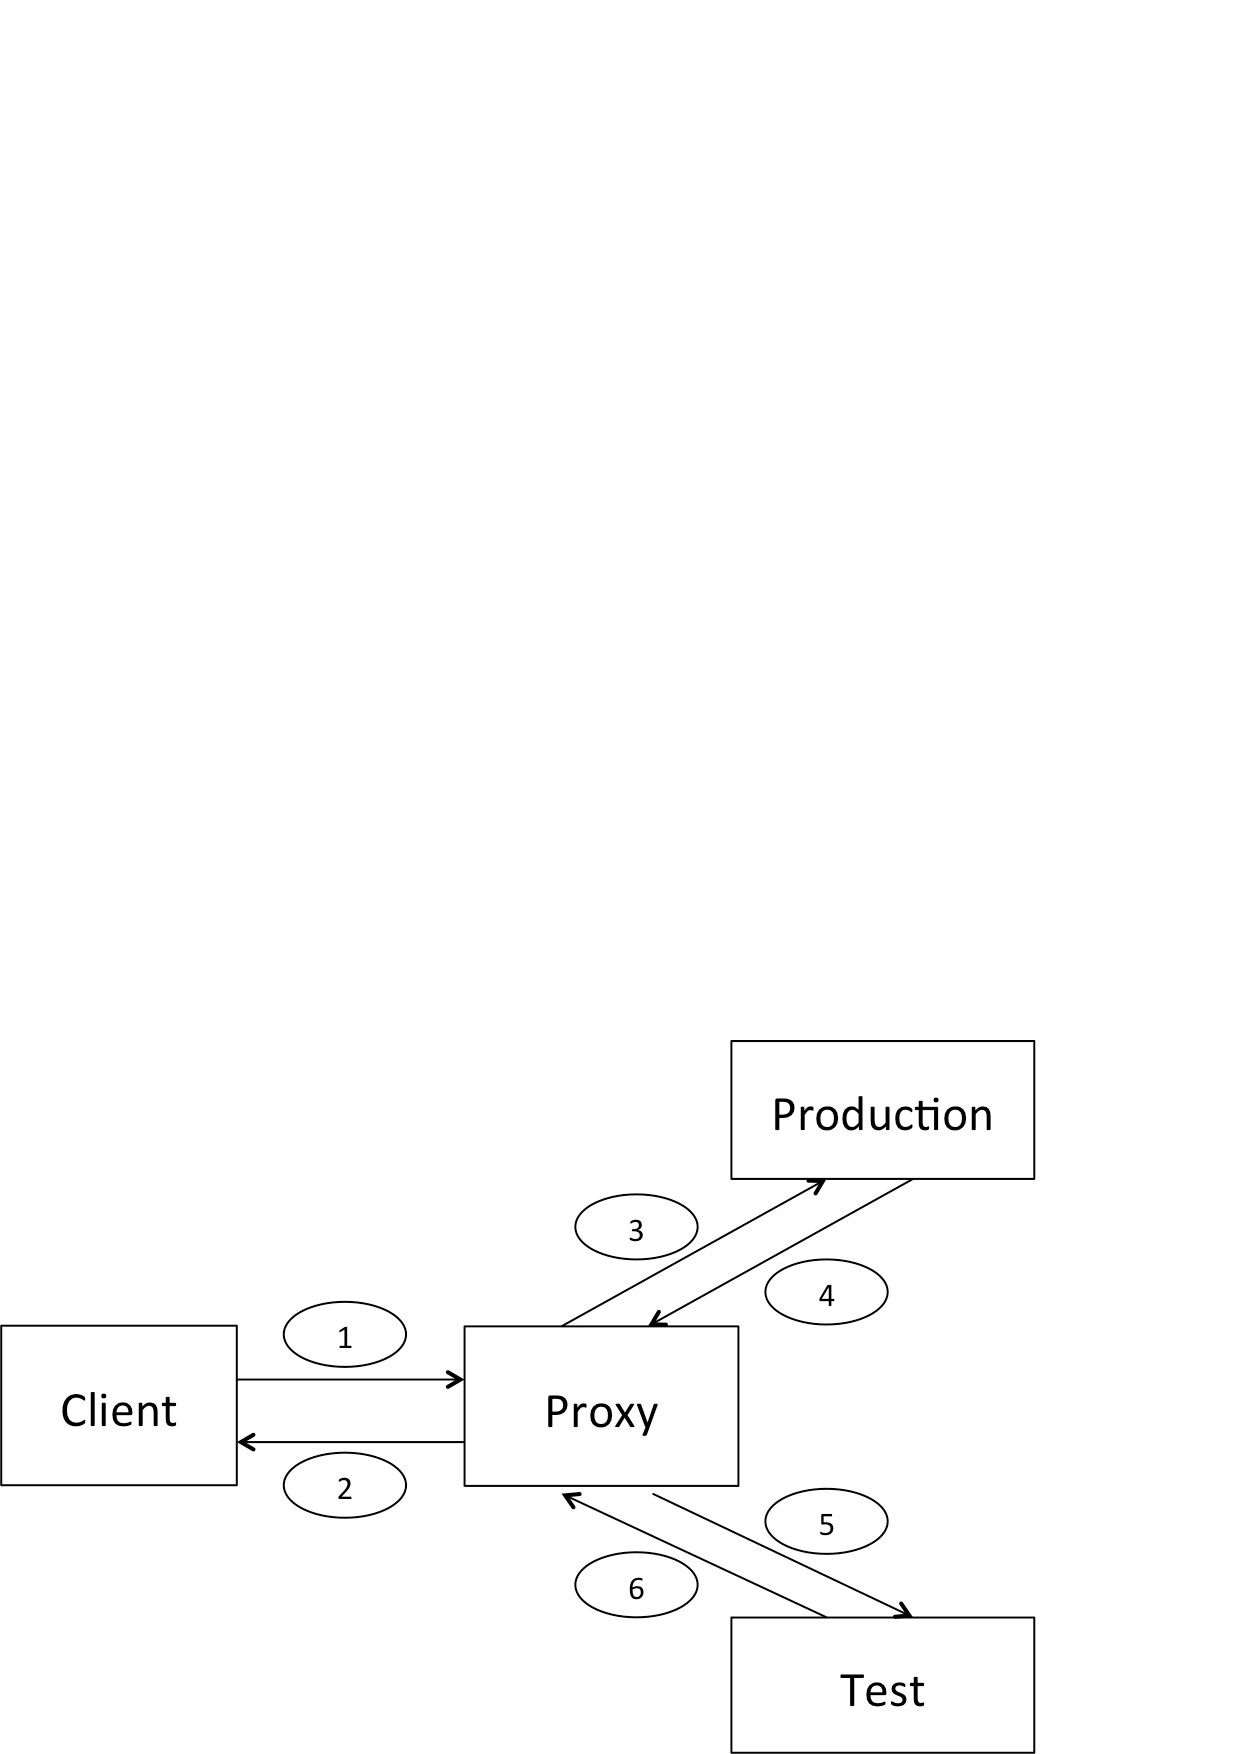
\includegraphics[width=0.4\textwidth]{figs/network_dup.pdf}
%    \captionsetup{justification=centering}
    \caption{Description of the Network Duplicator. In \textit{synchronized} mode: Thread 1 executes steps [1,3,5], and Thread 2 executes [2,4,6] sequentially. In \textit{asynchronous} mode: Thread 1 executes steps [1,3], Thread 2 executes [2,4], Thread 3 executes [5], and Thread 4 executes [6]}
    \label{fig:duplicator}
  \end{centering}
\end{figure}

\subsection{Proxy Network Duplicator} 
\label{sec:proxyDuplicator}

In order for \textit{live debugging} to work, both production and debug containers must receive the same input.
%This can be achieved in multiple ways, the easiest would be a port-mirroring mechanism either using software provided tap devices or in hardware switches (several vendors provide mirroring options). 
%These are both pretty common, and are blackbox and do not require much configuration.
%However, such port mirroring solution gives us minimal control on the traffic going to our test container.
A major challenge in this process is that the production and debug container may execute at different speeds (debug will be slower than production), which will result in them being out of sync.
Additionally, we need to accept responses from both servers, and drop all the traffic coming from the debug-container, while still maintaining an active connection with the client.
Hence simple port-mirroring and proxy mechanisms will not work for us.
%Hence a layer 2 level network solution is not possible as some context of the address and state are required

%Network proxies can be created at different levels in the network stack, for our purposes we have created a TCP proxy which mirrors the incoming traffic.
Our solution is a customized TCP level proxy, which also duplicates network traffic to the debug container, while maintaining the TCP session and state with the production container. 
Since it works at the TCP/IP layer, the applications are completely oblivious of it.
% and essentially works as a socket reader/writer which reads incoming TCP streams and writes these streams to two different socket connections for the production and test containers.
In this section, we discuss two strategies (we call \textit{duplication modes}) to duplicate and forward network traffic to the debug and production containers.
% we then explain a network aggregation mechanism which handles communication of the cloned debug-containers with upstream servers.  
%\begin{algorithm}[h!]
\caption{Network Duplication Algorithm}
\label{algoDuplication}

\scalebox{0.85}{
\begin{minipage}[t]{\linewidth}

\begin{algorithmic}
\State $prod\_port$: The port at which the production server is running
\State $test\_port$: The port at which the test container is running
\State $listen\_port$: The port at which the proxy is listening
\State $mode$: 1 -> synchronous packet forwarding, 2 -> asynchronous packet forwarding, 3 -> asynchronous load balanced packet forwarding
\\
\Function{main}{$prod\_port,test\_port,listen\_port$} 
\State spawn\_worker\_threads()  
\State bind(listen\_port) 
\State listen(listen\_port).on\_event(mode,prod\_port,test\_port) 
\EndFunction
\\
\Function{on\_event}{$mode, prod\_port, test\_port$}
\If {$mode==1$}
\State accept()
\State buffer=read\_input()
\State communicate\_production (buffer, prod\_port)
\State communicate\_test (buffer, test\_port)
\EndIf
\If{$mode==2$}
\State accept()
\State buffer=read\_input()
\State send\_to\_worker\_thread( communicate\_production (buffer, prod\_port))
\State send\_to\_worker\_thread( communicate\_test (buffer, test\_port))
\EndIf
\If{$mode==3$}
\State accept()
\State buffer=read\_input()
\State send\_to\_worker\_thread( communicate\_production (buffer, prod\_port))
\State send\_to\_worker\_thread( communicate\_test (buffer, test\_port))
\EndIf
\EndFunction
\\
\Function{communicate\_production}{$buffer, prod\_port$}
\State connect(prod\_port)
\State sendall(buffer)
\State sendToClient(recv())
\EndFunction
\\
\Function{communicate\_test}{$buffer, test\_port$}
\State connect(test\_port)
\State sendall(buffer)
\State recv()
\EndFunction
\end{algorithmic}
\end{minipage}
} % scalebox

\end{algorithm}


\subsubsection{Duplication Modes}
\label{sec:dupMode}

%\begin{enumerate}[leftmargin=*]
%\begin{enumerate}[leftmargin=*]

%\item 
\textbf{Synchronized Packet Forwarding Mode}: 
A naive strategy is to have a single worker thread to send and receive TCP stream to the production container as well as the debug container.
%This is the simplest strategy and is quite robust as far as sending proxy data is concerned. 
To understand this better let us look at figure~\ref{fig:duplicator}: Here each incoming connection would be handled by 2 parallel threads T1, and T2 in the proxy. 
Where T1 sends data from the client to the proxy (link 1), then sends data from proxy to production (link 3), and finally from proxy to debug container (link 5). 
Whereas, T2 sends replies from production to proxy(link 4), then receives replies from debug container to proxy (link 6), which are then dropped. 
Thread T2 then forwards packets received on link 4 to the client on link 2.

By design TCP is a connection oriented protocol and is designed for stateful delivery and acknowledgment that each packet has been delivered.
Packet sending and receiving are blocking operations, and if either the sender or the receiver is faster than the other the send/receive operations are automatically blocked or throttled.

This can be viewed as follows: Let us assume that the client was sending packets at $X Mbps$ (link 1), and the production container was receiving/processing packets at $Y Mbps$ (link 3), where $Y<X$. 
Then automatically, the speed of link 1 and link 2 would be throttled to $Y Mbps$ per second, i.e the packet sending at the client would be throttled to accommodate the production server. 
Network throttling is a default TCP behavior to keep the sender and receiver synchronized.
%This behavior adheres to the default TCP protocol.
%, and if our proxy was only forwarding traffic to the production container it would be fine.
However, we also send packets to the debug-container (link 5) in the same sequential thread T1. 
Hence, if the speed of link 5 is $Z$ $Mbps$, where $Z < Y$, and $Z < X$, then the speed of link 1, and link 3 would also be throttled to $Z$ $Mbps$.

%Such a communication model effects the user-experienced delay for the targeted SOA application, and is against the guiding principal of \parikshan.
The speed of the debug container is likely to be less than the production container, hence this would definitely impact the performance of the production container.
Clearly, this is a non-optimal solution. 
Next we discuss an asynchronous packet forwarding scheme, which avoids any slowdown to the production container.

%It especially works well with standard SOA architectures with small incoming packet flows, 
%as it means that the delay caused in the test and production container would be minimal.
%However, a major disadvantage of this approach is that every connection received would 
%finish a round trip connection with production container before sending the packets to the test-container.
%This would obviously delay all communication to the test-container by the amount of time it takes for the production container to respond. 
%However, more importantly it also effects the speed of the production container for every subsequent flow, 
%since it will have to wait for the time taken to send the packets to the test container.
%We assume a worker thread model for our proxy, where each connection is managed separately by one worker thread, 
%since our target is a service oriented architecture there should be frequent small connections from multiple users, hence a threading model is important.

%\item 
\textbf{Asynchronous Packet Forwarding Model}: 
%In the synchronized mode the debug container, can impact the speed of the production container as well. 
%The main reason for this is because of blocking sends being used to forward packets from the client to the debug-container and production container by the same sequential process.
In the asynchronous packet forwarding mode (see figure \ref{fig:duplicator}): we use 4 threads T1, T2, T3, T4 to manage each incoming connection to the proxy.
Thread T1 forwards packets from client to proxy (link 1), and from proxy to production container (link 2). 
It then uses a non-blocking send to forward packets to an internal pipe buffer shared between thread T1, and thread T3. 
Thread T3, then reads from this piped buffer and sends traffic forward to the debug-container. 
Similarly Thread T2, receives packets from production container, and forwards them to the client, while Thread T4, receives packets from the debug-container and drops them.

The advantage of this strategy is that any slowdown in the debug-container will not impact the production container's communication as a non-blocking send is used to forward traffic to the production container. 
A side-effect of this strategy is that if the speed of the debug-container is too slow compared to the production container, it may eventually lead to a buffer overflow. 
We call the time taken by a connection before which the buffer overflows it's \emph{debug-window}.
We discuss the implications of the \emph{debug window} in section \ref{sec:window}.  
%In this strategy we have two worker threads which simultaneously handle sending and receiving tcp streams for the production container as well as the test container.
%Whenever any event happens the connection is established, and the incoming message is read to a buffer, this buffer is then sent to a worker thread for forwarding the data to the production container, and another thread for forwarding the data to the test container. 
%This means that unlike our previous model, the processing time of either the production container or the test container will not effect the performance of the other.
%We have a slightly modified worker thread model, in which each incoming connection is managed by two worker threads one for communication with the production and the other for the test.

%\item \textbf{Asynchronous Load Balanced Packet Forwarding Model}

%It is still possible that there will be slowdown, and a short packet window because of the overhead of running test-cases in the test container. 
%This would mean that the test container will have a short time-window to execute test-cases.


%\end{enumerate}

%The algorithm for each of the packet forwarding modes has been described in Algorithm.\ref{algoDuplication}. 
%As an added explanation, the only difference between communication with the production container v/s the test container is that the when the proxy receives the message back from the production container, it sends the stream back to the client, on the other hand for the test container the packets are simply received and then dropped.


\iffalse

Since the speed of input from the client is not in sync production-container, we need to buffer incoming traffic and relay it to the the TCP Connector(Node 6, figure \ref{fig:duplicator}) as soon as the test-container is ready for new traffic. 
Since parallel connections can be initiated by the client on the same TCP port, the Buffer-Manager creates multiple buffers for each connection, and initiates new connections by following the same causal flow of the packets received from the client. 
Unlike record-replay systems \parikshan does not claim to have strong consistency requirements, and does not need to exactly follow the production container as the goal is not reproduce all non-determinism in the production environment, but instead capture input non-determinism, and complete system state from a given point of time.
We discuss consistency requirements further in section \ref{sec:consistency}

\fi

\begin{figure}[ht]
  \begin{center}
    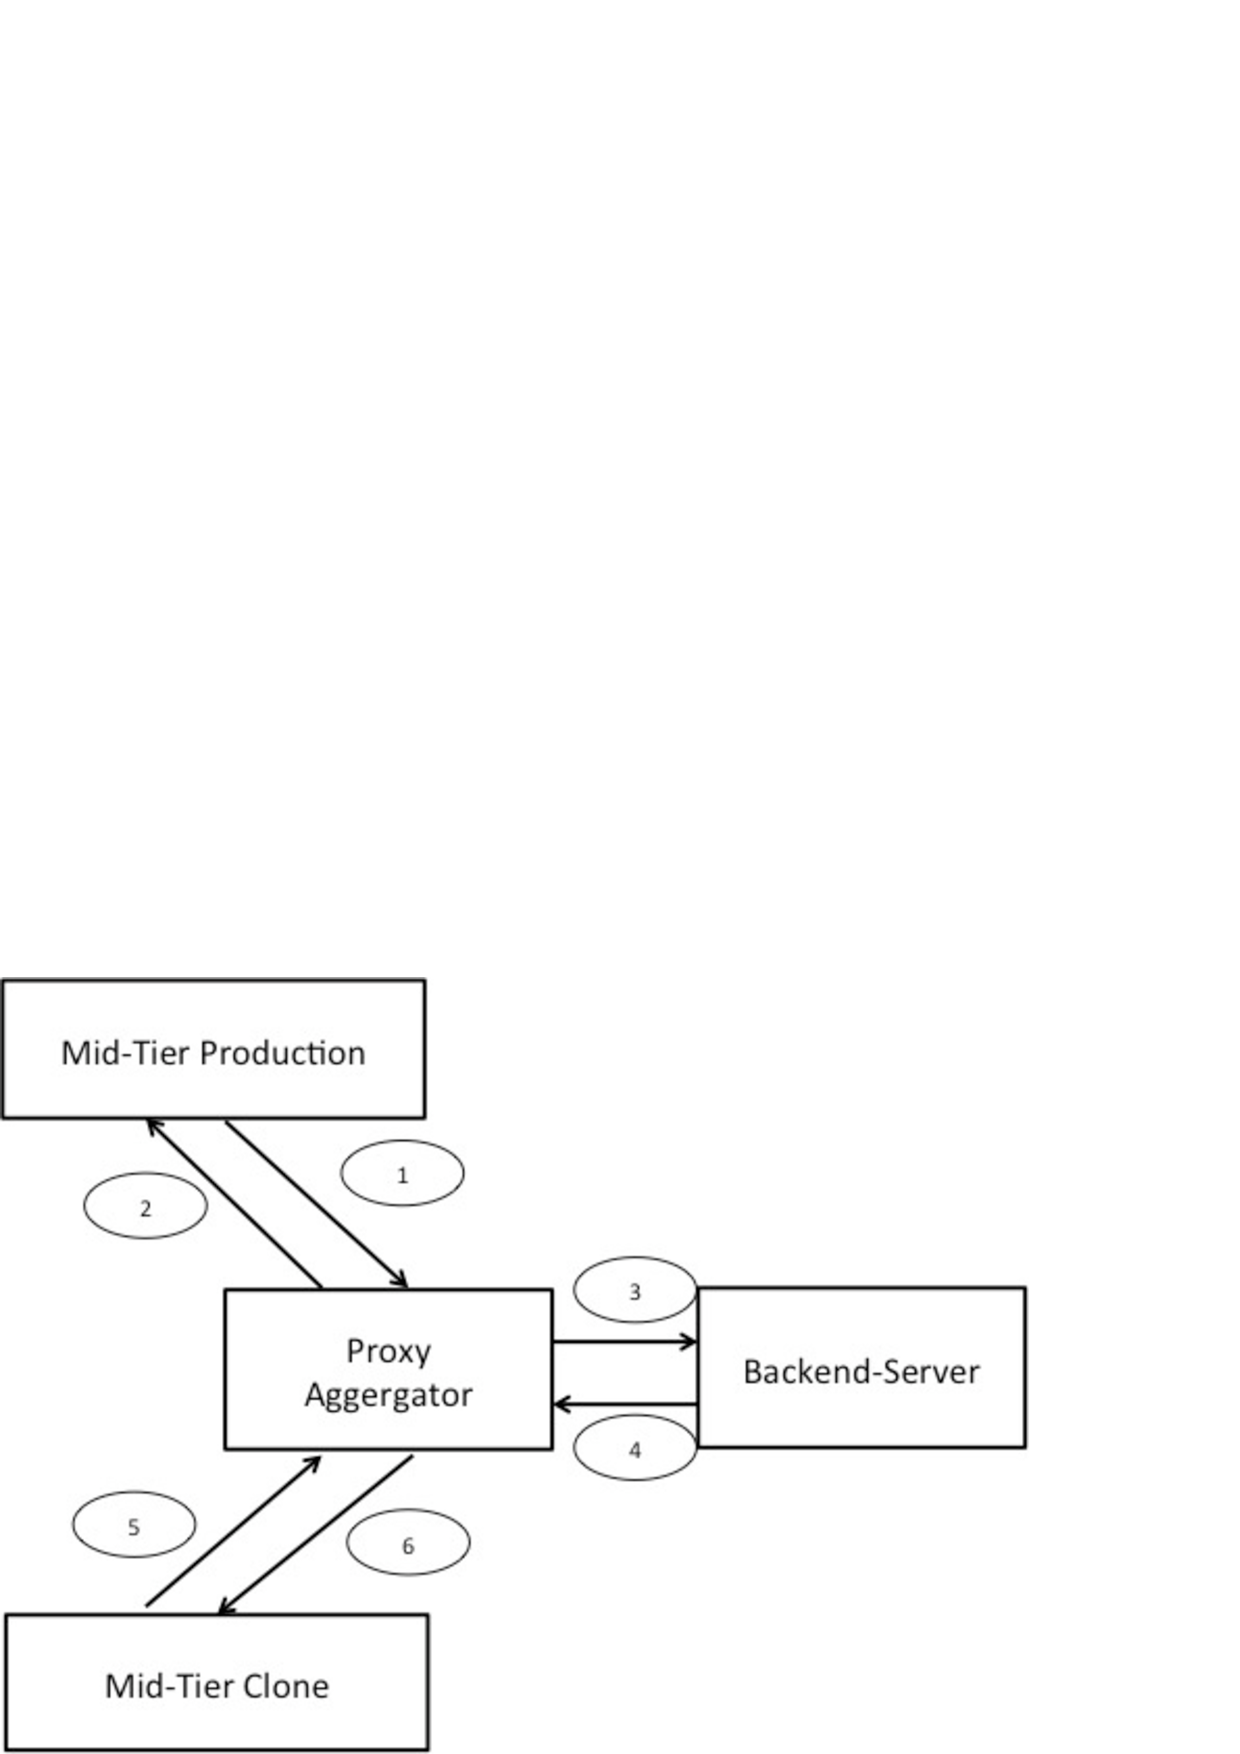
\includegraphics[width=0.6\textwidth]{figs/aggregator.pdf}
%    \captionsetup{justification=centering}
    \caption{Description of the Network Aggregator. Thread 1 executes step [1,3], Thread 2 executes [2,4], and Thread 3 executes [5], and Thread 4 executes [6]}
    \label{fig:aggregator}
  \end{center}
\end{figure}

\subsection{Proxy Network Aggregator \& Replay }
\label{sec:proxyAggregator}
The proxy described in section~\ref{sec:proxyDuplicator} is used to forward requests from downstream tiers to production and debug containers.
This manages incoming ``requests'' to the target container, however the same mechanism cannot be directly applied for isolating responses from upstream servers.
Imagine if you are trying to debug a mid-tier application container, the proxy network duplicator will replicate all incoming traffic from the client to both debug and the production container. 
Both the debug container and the production, will then try to communicate further to the back-end containers.
This could mean duplicate queries to the backend servers (for e.g. duplicate deletes to MySQL), thereby leading to an inconsistent state.
However, to have forward progress the debug-container must be able to communicate and get responses from upstream servers.
The ``proxy aggregator'' module stubs the requests from a duplicate debug container by replaying the responses sent to the production container, to the debug-container.
As well as dropping all packets sent from it to upstream servers.

As shown in  Fig~\ref{fig:aggregator}, when an incoming request comes to the aggregator, it first checks if the connection is from the production container or debug container. 
In case of the production container (link 1), the aggregator forwards the connection to the backend (link 3), responses from the backend are sent to the aggregator (link 4), and then forwarded to the production container (link 2) and simultaneously saved in an internal queue.
The aggregator creates an in-memory persistent inter-process FIFO queue for each connection where the responses for each of these connections are stored.
When the corresponding connection from the duplicate debug container connects to the proxy (link 5); all packets being sent are quietly dropped. 
The aggregator then uses the queue to send replies to the debug-container (link 6).
In a way this is a streaming online record-and-replay, where we are recording the data in our buffer.
We assume that the production and the debug container are in the same state, and are sending the same requests. 
Hence, sending the corresponding responses from the FIFO stack instead of the backend ensures: (a) all communications to and from the debug container are isolated from the rest of the network, (b) the debug container gets a logical response for all it's outgoing requests.

In this design we assume that the order of incoming connections remains largely the same.
We use a fuzzy checking mechanism using the hash value of the data being sent to correlate the connections. 
Each queue has a short wait time to check against incoming connections, this allows us to match slightly out of order connections.
In case a connection cannot be correlated, we send a TCP\_FIN, to close the connection, and inform the debugger.
We believe that this should be relatively rare.
Furthermore, since we are looking into SOA applications, each user request is technically a seperate thread and should have minimal impact on other requests. 
Hence killing a small percentage of requests which could not be correlated, should not have a drastic impact on the status of the status of the debug container as compared to the production container. 
To further insure the debug container fidelity, we have an optional divergence checking mechanism explained in section~\ref{sec:divergenceChecking}.
%In case a connection cannot be correlated, we allow the connection to time out and send a TCP\_FIN.

\subsection{Debug Window}
\label{sec:window}

%At the time of the live cloning, the testing container has an identical status and receives the same input as the production container. 
%Hence, any test-cases run in the testing container, should faithfully represent the status of the production container.
%However, an obvious down-side to any debugging/testing is that it will add an overhead on the performance of the test-container as compared to the production environment.
%This would mean that the execution of requests in the test-container will lag behind the production container. 
%To avoid this slowdown impacting the actual production container, 
%\noindent
In the asynchronous forwarding mode, an unblocking send forwards traffic to a separate thread which manages communication to the debug-container. 
This thread has an internal buffer, where all incoming requests are queued, and subsequently forwarded to the debug-container. 
The incoming request rate to the buffer is dependent on how fast the production container manages the requests (i.e. the production container is the rate-limiter).
Whereas the outgoing rate from the buffer is dependent on how fast the debug-container processes the requests.
Because of instrumentation overhead in the debug-container, the outgoing rate is likely to be less than the production container.
The time period till buffer overflow happens is called the \emph{debug-window}.
This depends on the size of the buffer, the incoming request rate, and the overhead induced in the debug-container. 
For the duration of the debugging-window, we assume that the debug-container faithfully represents the production container. 
Once the buffer has overflown, the production container may need to be cloned again to ensure it has the same state.

%\noindent
The debug window size also depends on the application behavior, in particular how it launches TCP connections. 
\parikshan generates a pipe for each TCP connect call, and the number of pipes are limited to the maximum number of connections allowed in the application.
Hence, buffer overflows happens only if the requests being sent in the same connection overflow the queue.
For webservers, and application servers, the debugging window size is generally not a problem, as each request is a new ``connection'', hence the proxy is able to tolerate significant slowdowns.
Database servers, and other session based services usually have small request sizes, but multiple requests can be sent in one session which is initiated by a user. 
In such cases, the amount of calls in a single session can eventually have a cumulative effect to cause overflows.
Photosharing, file sharing and other datasharing services transfer a lot of data in a single burst over each TCP connection. 
These protocols will have an overflow relatively sooner, and will be able to tolerate only small amounts of slowdown. 

To further increase the \emph{debug window}, we propose load balancing debugging across multiple debug-containers, which can each get a duplicate copy of the incoming data. 
This would mean that there are multiple threads handling the incoming connection, one for the production container, and one for each of the debug containers.
We believe that such a strategy would significantly reduce the chance of a buffer overflow in cases where the debug-container is significantly slower.
We evaluate debug-window overflows in section~\ref{sec:timewindowPerformance}.

%\iffalse
%In this section we try to model the testing window by using concepts well used in queuing theory(for the sake of brevity we will avoid going into too much detail, readers can find more about queuing theory models in~\cite{queueWiki}).
%The buffer overflow of our test-container can be modeled as a M/M/1/K queue (Kendall's notation~\cite{kendall}), for our simplest asynchronous model, and as a M/M/c/K queue in the asynchronous load-balanced model.
%An M/M/1/K queue, denotes a queue where requests arrive according to a poisson process with rate $\lambda$, that is the inter-arrival times are independent, exponentially distributed random variables with parameter $\lambda$ . 
%The service times are also assumed to be independent and exponentially distributed with parameter $\mu$. Furthermore, all the involved random variables are supposed to be independent of each other. 
%Further, the notation specifies that there are $c$ queues/ or alternatively $c$ servers managing the requests, and the queues is of a finite capacity, i.e. the queue can accommodate a maximum of K requests.
%In our case $\lambda$ denotes the rate at which requests arrive to the buffer from the production container, and $\mu$ denotes the processing time overhead of each request in the test-container (to simplify the problem, we ignore the actual processing time of the test-container, as the incoming rate $\lambda$ is already synchronized with the production container processing time, and it is only the overhead added by the test-container which matters). 
%In our simple asynchronous forwarding strategy, we have $c=1$ as we have only a single test-container, potentially as explained earlier, in a load-balanced asynchronous model this could be extended to $c$ servers to increase the time window.

%Now based on this notation the expected size of the time window is :
%\texttt{Nipun's note - This equation and is tied to the evaluation in section 7.2, which is being worked on}
%\fi


%In queueing theory terms, the size of the testing window can be modelled as a special case of continuous-time Markov process also called the \emph{birth-death} process. 
%For the sake of brevity we will only briefly explain the basics of queueing theory
%It is possible that in heavy load conditions the buffers in the Buffer Manager may overflow. 
%Depending on the use-case the BufferManager can then trigger the CloneManager, which closes the analysis time-window and launches a fresh clone.
%Incoming traffic may potentially have a cumulative effect which will eventually lead to a buffer overflow in the BufferManager, hence leading to packet drops, and eventually leading to a modified state in the testing container, which can no longer faithfully represent the production container.
%This behavior is similar to packet dropping in classical TCP buffers, which rely on re-transmission of incoming packets from the client.
%However in our case if packets are dropped the client cannot re-transmit them as it not in sync with the test container.
%Hence in some cases \parikshan analysis, has to be restricted to a time-window dependent on the load of incoming traffic and the slowdown experienced by the test-container.

%Let the rate of incoming traffic be \lambda


\subsection{Divergence Checking}
\label{sec:divergenceChecking}

%\textbf{Divergence checking}: 
%As mentioned earlier, we clone the entire state of the production container, and replicate the incoming requests. 
%We believe that this should capture most non-determinism in the application, and the debug container should be a close representative of the production container. 
%However, 
%\noindent
It is possible that the behavior of the production and debug container may diverge with time.
To understand and capture this divergence, we compare the corresponding values of tcp send and receive within the proxy.
This component is optional and it gives us a black-box mechanism to check the fidelity of the debug-container.
Comparisons are based on hash of the data packets, which are collected and stored in memory for the duration that the connections are active.
The degree of acceptable divergence (the point till which the production and debug containers can be assumed to be in sync) is dependent on the application behavior. 
For eg. an application which is sending timestamps in each of it's send messages can be expected to have a much higher degree of divergence, in comparison to an application which is querying a database.



\iffalse
\subsection{Network State Model}
\label{sec:networkStateModel}

Network communication in most applications consists of two core types of protocols: UDP \& TCP.
The UDP(User Datagram Protocol) allows the applications to send messages(referred to as datagrams) to other hosts in the network without prior communications to set up any transmission channels.
UDP uses a simple communication mechanism while minimizing protocols. 
It has no handshaking dialogs or acknowledgment of package delivery. It is broadly used for network traffic where speed is much more important than reliability (viz. network streaming applications like video etc.)
On the other hand TCP(Transmission Control Protocol) is a reliable error checked delivery stream.
It involves initially establishing the connection, and allowing for packet re-delivery or re-ordering to allow for reliable and dependable connection. 
While TCP is slower than UDP it is preferred for most normal connections between clients and server applications.

Since the UDP protocol has no error management mechanism, it automatically follows that machine state in a UDP connection is not important.
Hence in our design the duplicator can easily flood packets to the cloned UDP server by simply sending packets to the targeted host and port. 
Our solution for this is 
\fi
\iffalse
\begin{figure}[!ht]
  \begin{center}
    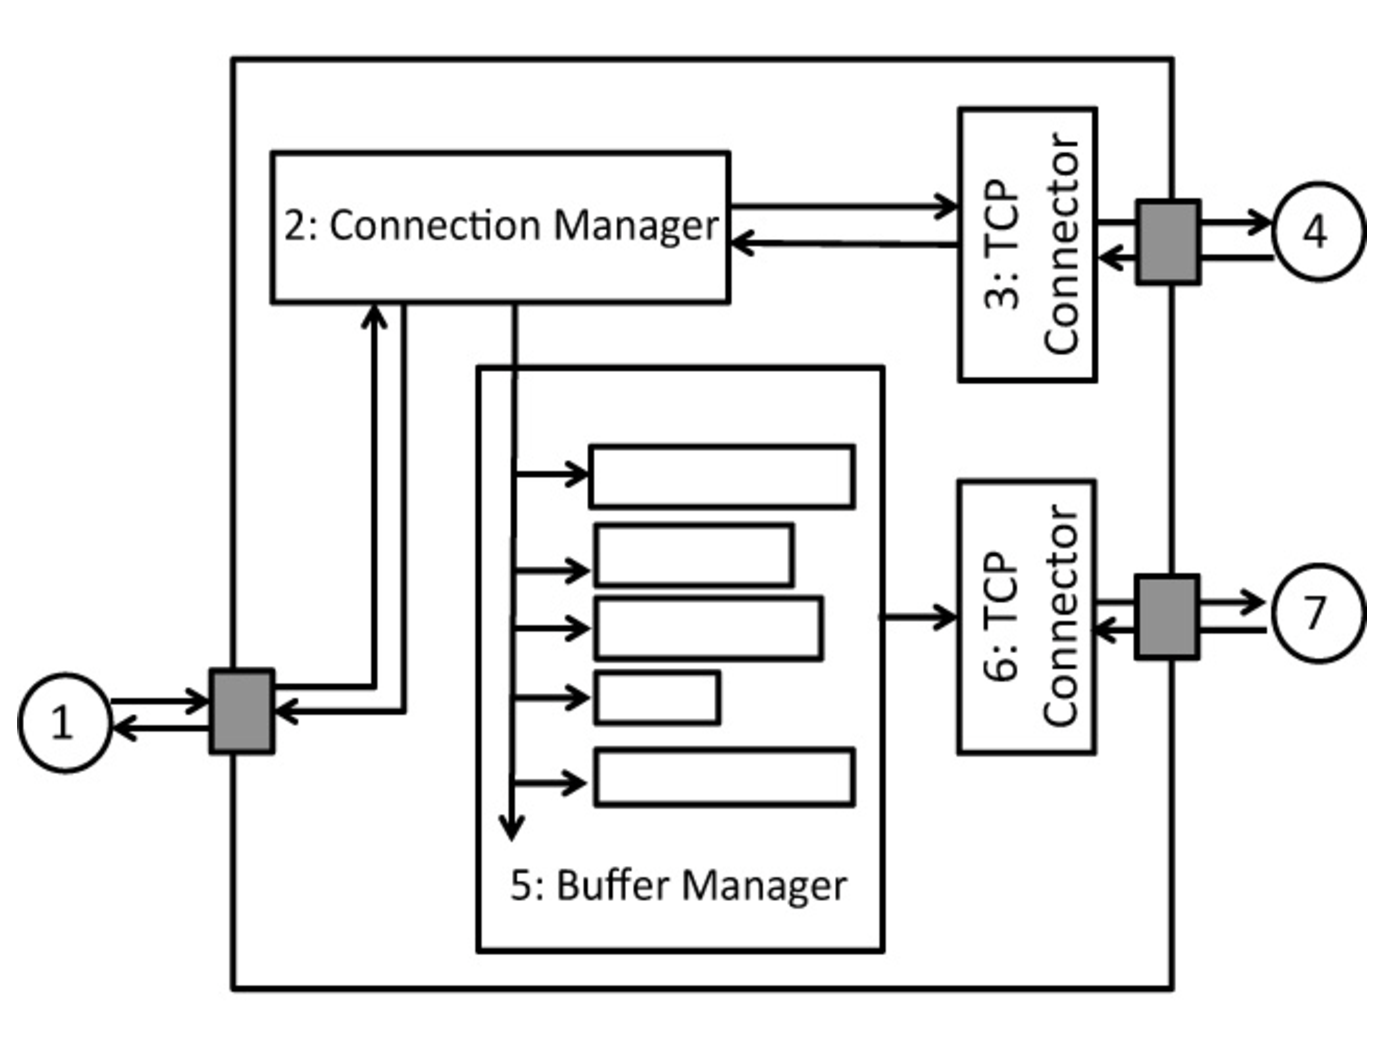
\includegraphics[width=0.5\textwidth]{figs/duplicator.eps}
    \caption{Description of the Network Duplicator}
    \label{fig:duplicator}
  \end{center}
\end{figure}

The workflow of each component is as follows: Traffic from the client (Node 1 in figure \ref{fig:duplicator}) is forwarded to the Connection Manager (Node 2 in figure \ref{fig:duplicator}). 
The connection manager essentially is a socket reader which copies, parses the incoming traffic. 
Based on the type of TCP request, a new connection is created or data is forwarded/received to/from the TCP Connector( Node 3, figure \ref{fig:duplicator}) which in turn creates a connection to actual production server.
In this way the connection manager and TCP connector follow the TCP state machine hence maintaining network packet sanity while forwarding traffic to the production container.
Simultaneously, the connection manager creates an internal copy of incoming traffic, and parses and sends it to the Buffer Manager (Node 5, figure \ref{fig:duplicator}).
\fi


\section{Implementation}
\label{sec:implementation}

%\noindent
%\parikshan is built on top of user-space container virtualization software, OpenVZ~\cite{openvz}, with Centos 6.5 with Linux Kernel 2.6.32.
%Each container disk layout uses ploop~\cite{ploop} devices to enable faster and easier cloning.
%The OpenVZ functionality, was extended to enable live-cloning as explained in section \ref{sec:design}.
%We modified and used the OpenVZ toolkit vzctl version 4.8 to create our cloning, creation and destroy scripts for the container. 
%While the technology has also been tested on Debian systems, the evaluation in this paper has been done on RHEL(Centos) Systems. 
%For our evaluation, we have not put in resource restriction on the containers (i.e. the containers have access to the same hardware resources as the host machine).
%Users using \parikshan may put resource restriction as required.
%\parikshan also requires a number of commonly available linux modules to allow for network connectivity and 
%\noindent
\parikshan is built on top of user-space container virtualization software, OpenVZ~\cite{openvz}, with Centos 6.5 with Linux Kernel 2.6.32.
We implemented the system in 3 different configurations: 
(1). We applied \parikshan 's internal mode configuration by installing it in a single host OS VM with Intel i7 CPU, with 4 Cores, and 16GB RAM. 
%\parikshan was installed on multiple VM's running on the host OS using KVM based virtualization. 
Containers were cloned within the machine, with a seperate VM acting as the client.
We used NAT, and IP namespaces for network access to the VM's.
(2). We impelemted our system's external mode on the base kernel in identical host nodes. 
Each of these host nodes have an Intel Core 2 Duo Processor, 8GB of RAM, and ran Centos 6.5 with Linux Kernel 2.6.32.
%(3). To verify our implementation in a enterprise level public cloud provider, we also implemented a prototype on Google's Cloud Infrastructure (Google Compute~\cite{gcompute}).
%The production and the debug container's were run on different virtual nodes, with 2 VCPU's and 4G RAM. 
%The main advantage of using the Google Compute Engine was to run our cloning scripts on real data-centers, and also to scale out our evaluation. 

The network proxy was implemented in C/C++.
The forwarding in the proxy is done by forking off multiple processes each handling one send/or receive connection in a loop.
Data from processes handling communication with the production container, is  transferred to those handling communication with the debug containers using pipes.
Pipe buffer size is a configurable input based on user-specifications. 
\section{Triggering and Inserting Analysis}
\label{sec:trigger}

The key idea behind sandbox testing is to ofcourse insert test-cases 
Once we have forked off a clone, we are now ready to do some deeper analysis. 
%By design, \textit{Parikshan} can allow a variety of test cases. 
We divide such analysis in two parts based on the time window required for analysis: (1).Statistical

\subsection{Inserting Probes \& TestCases}
\label{sec:unitTests}

Inserting probes in the sandbox can be done using existing dynamic instrumentation

\subsection{Statistical Analysis}
\label{sec:statisticalTests}

Analysis which need a long time window to record, and run the status across multiple requests are considered as long running analysis. 
Such analysis can be considered to be similar to monitoring of live applications, and are usually statistical in nature.
Typically tools such as PIN \cite{pin}, Valgrind \cite{valgrind}, Dyninst \cite{dyninst}, can do deep analysis without modifying the logic of the application.
However, they impose a heavy penalty in terms of performance.
Such tools can be easily used in \textit{Parikshan}, without effecting system performance.
However, there are a few challanges with such statistics which need a longer window to run.


%\section{Network Issues}
\label{sec:network_issues}

There are several problems that can effect the execution of sandbox testing. 

\begin{itemize}
  \item \textbf{Stateful Connections}
  \item \textbf{Time Lag}
\end{itemize}

\section{Early Validation}
\label{sec:evaluation}

%In this section we present the evaluation of \parikshan. 
%The key questions facing us were:
%\begin{itemize}
%  \item How can \parikshan be used in the real world? 
%  \item Does the test container faithfully represent the execution and the state of the production container? 
%     \item How does cloning the container effect the performance of the production container?
%     \item How long of a testing-window do we have? 
%   \item How does running tests in the test-container effect the performance of the production container?
%\end{itemize}

%In order to answer these questions, we separated our evaluation in looking at two different stages: cloning stage, time-window analysis.

%\subsection{Cloning: Micro-Benchmarks}
%\label{sec:performance}

\begin{table}[ht]
  \centering
    \begin{tabular}{ | p{1.8cm} | l | l | l | l |}
    \hline
    \textbf{Modes} & \multicolumn{2}{|c|}{\textbf{Internal Mode}} & \multicolumn{2}{|c|}{\textbf{External Mode}}\\\hline
    \textbf{ } & \textbf{Cloning} & \textbf{Hog+Cloning} & \textbf{Cloning} & \textbf{Hog+Cloning} \\ \hline
    \hline
    \textbf{Throughput} & --  & 1509 req/s & --  & 625\\ \hline
    \hline
    \textbf{Suspend + Dump} & 0.49 & 0.46 & 0.10  & 0.10\\ \hline
    \textbf{Pcopy } & 0.22  & 0.27 & 0.44  & 0.39\\ \hline
    \textbf{Copy Dump } & 0.62  & 0.64 & 0.28  & 0.31 \\ \hline
    \textbf{Undump} & 1.33  & 1.53 & 0.84 & 1.03 \\ \hline 
    %\textbf{--------------} & --- & --- & --- & --- & --- & --- & --- & --- & --- \\ 
    \hline
    \textbf{Suspend Time} & 2.66 & 2.91 & 1.67 & 1.83 \\ \hline
    \end{tabular}
    \caption{Performance of container cloning suspend time in external vs internal modes, when running httperf webserver hog workload.
      The hog processes 1601 req/s without any cloning in the internal mode, and 675 req/s in the external mode}
\label{table:clonePerf}
\end{table}

%The profile of the cloning operation can be divided in 4 stages: 
%(1) Suspend \& Dump: this is the time taken to suspend the container, 
%(2) Pcopy after suspend: which does the rsync after the suspend of the file system of the container, 
%(3) Copy Dump File: which copies the process state, and finally 
%(4) Undump and Resume: which is the time taken to resume the containers. 

\noindent \textbf{ Q1: How does cloning impact production systems and how fast is cloning?  }
In Table \ref {table:clonePerf}, we show the suspend times when cloning a production container (webserver) that is idle vs. a container which is running an Apache hog benchmark \cite{httperf} on it. 
The first column gives the average performance of the cloning operation without any hog operation running on it.  
An idle or a container with minimal processing is cloned relatively fast: 2.66 seconds on the idle container. 
We then tried to run an Apache hog to make a baseline of Apache's performance without cloning, and found that a page fetch gave us a throughput of 1601 req/s (internal mode). Then we tried to do cloning of the same container while running the hog, and found minimal change (1509 req/s) in the performance of the hog, and very little impact on the suspend time of live cloning.
The key thing to note in these experiments was that we \textbf{did not have any connection failure or connection refused, and only a slight decline in the throughput during the cloning operation}. 
At the application layer, the TCP packet drops are hidden as packets are resent from within the TCP protocol.
%To further investigate the tcp packet dropping, we ran an iperf\cite{iperf}( a tool to measure tcp benchmark) server while cloning the production container. 
%We were indeed able to observe packet dropping for about 2 seconds in the iperf client, however, the important point to note is that there were no requests dropped for the application while doing cloning. 
\iffalse
\begin{figure*}[t]
	\begin{center}
		\includegraphics[width=1\textwidth]{figs/fioResult.png}
		\caption{Comparison between cloning between the internal vs external mode, while continuously increasing the file write operations to disk}
		\label{fig:fioResults}
	\end{center}
\end{figure*}
\fi
%As explained earlier, the cloning process can be divided into two parts: an rsync operation which does an ``pre-copy'' of the VM, and a follow-up rsync operation while the target container is suspended, to make sure that both the production and test containers have the exact same state.
%The idea is to reduce the time taken to suspend the production container, so that it has minimal effect on the user.

\noindent \textbf{ Q2: What factors effect cloning performance? }
The main factor that effects suspend time is the number of ``dirty pages'' in the suspend phase, which have not copied over in the pre-commit rsync operation.
%Naturally, the number of write operations in the container while cloning the container, will increase the number of dirty pages, and increase the time of the suspend operation.
%To understand the effect that I/O operations have on the cloning operation, we ran a controlled experiment gradually increasing the number of I/O writes and writes. 
We use fio(flexible io tool for linux)\cite{fio}, to increase the number of I/O operations while doing cloning. 
%Specifically, we do random-write operations of a 500MB file with fixed i/o bandwidth rates.
%As shown in figure \ref{fig:fioResults}, i
In our experiments with a read intensive workload, the suspend time was about 3-4 seconds, with upto 2-3 Mbps of read I/O. 
In essence, we found that read operations do not really impact the performance of our cloning. 
On the other hand for write operations, cloning has minimal impact for write I/O bandwidths of about 100Kbps - 150 Kbps operations. 
However, it increased rapidly beyond that. Thus, the increased cloning time confirmed our intuition that the cloning operation will be impacted when running a write I/O intensive application.
.
%Here we also compare the performance of cloning in the internal mode vs the external mode, while showing the time taken in various stages of cloning.
%While for lower I/O operations, the performance of both were similar, as we go higher, the external mode which uses the network to transfer the dirty pages during the cloning operations becomes a bottleneck. 
%The internal mode is much faster as both the production and test-container are hosted in the same physical device, so they have a much higher bandwidth between them.
%We can also see that the majority of the time is spent in pcopy after suspend, which is doing the copy of the dirty bits after suspend, especially for higher I/O's the other operations become negligible in comparison.
We would like to point out here, that most SOA application are usually read or CPU intensive operations, and several studies have shown live migration performance to be acceptable\cite{vmperformance} for most application SLA's. 
To conclude, we validated that live cloning generally takes less than two seconds  and is not disruptive to application clients (there is no loss of service visible). 
However, in high I/O write intensive workloads, the amount of time taken to clone can reach one or two minutes.
In such cases, we did observe retries and the performance of the server did suffer. 
Rate-limiting in the proxy can possibly be applied as a mitigating mechanism to allow for reduced suspend time in cloning. 
Alternatively some migration approaches use many more iterations or network-page faults, to reduce the suspend time further. For sake of brevity we do not discuss them here.

\iffalse
\textbf{Case-Study: } we debugged some real bugs such as mysql bug 18511 \cite{mysqlbug}, and did performance profiling of PetStore a 3 tier J2EE e-commerce system. 
We were able to increase the instrumentation sufficiently to debug the system within the test-container, by first doing a function level execution trace, and then adding a breakpoint at suspiciously long executions.
Using debugging and instrumentation tools, we were able to localize the bug to a highly non-optimal string matching for japanese, and chinese characters.
Simultaneously we observed no performance degradation in the production system.
%Current research in live migration has looked into further decreasing the sync time by doing active migration, and trigger page fault for the dirty bits which were not copied over.
%This is a similar to a copy-on-write method, that could possibly reduce our suspend time.
%In the interest of time, we have not explored faster means of live cloning, but aim to do so in our future work.
%However, it would impact, the overall performance of both systems as it would do the rsync operation for a much longer time-period.
\fi
\iffalse
\subsection{Time-Window Size Evaluation}
\label{sec:timewindowPerformance}

As explained in section \ref{sec:timewindowPerformance} if the overhead of the test-container is too high, the buffer may overflow.
This indirectly means that the test-container and the production-container are potentially out of sync.
In our current design we re-initiate the test-container by cloning again, and we call the time taken to reach a buffer overflow the "time-window" for the test-container.
As explained earlier, the size of this test-container, depends both on the overhead of the "test"/"instrumentation", as well as the incoming workload.

In this section we evaluate the testing window size using varying amounts of instrumentation, and the workload.
For the purpose of this evaluation, we keep a fixed buffer size. 
First we use a controlled workload rate, and gradually increase the overhead, then we use another scenario, where we keep the try to keep the same overhead, and try to increase the workload.
We also use real-world network packet capture data, to simulate a realistic workload and gradually increase the overhead there

\texttt{Nipun's note: This section still needs to be completed, I'm finishing up some of the results, before I can generate the charts}

\subsection{Overhead while Running tests}
\label{sec:overhead}

One of the most important goals of using \parikshan is to allow debugging without having any overhead on the actual application.
In this section we verify that this goal of \parikshan holds true i.e. debugging in the sandbox-container, does not effect the performance container. 
To understand the effect we ran some tests on our cloned container, with an independent cpu hog (infinite while loop with sleep) running within the test.
We gradually increased the amount of cpu being used by the cpu hog and found that while in the external mode there is no effect on the performance of the production container, in the internal mode at higher cpu hog percentages, the throughput of the production container is reduced.
This was an expected result, as the production container and test-container time share resources on the same machine, whereas in the external mode, they are completely isolated.
However, it is to be noted, that most debugging scenarios are unlikely to be cpu hogs, and if resource management in the container level is done properly, the containers in the internal-mode can be largely isolated from each other.

\fi


%Parikshan enables the users to freely run any test-case in the test-container while not effecting the production container. 
%At the same time the output of these tests should not effect the functionality or the performance of the production system.
%The main advantage of such a system can be seen in service oriented applications which are user facing and can hence ill-afford to be shutdown for inspecting bugs.
%As mentioned earlier, another major advantage is that we are able to capture live user-input. \\

%\par \noindent
\section{CaseStudy: Debugging using Execution Tracing of MySQL bug 15811}  
%Performance profiling such as function execution trace, execution time, resource usage etc., is often used to indicate and localize performance bugs in real world systems. 
%While performance profiling is simple to implement, it obviously incurs an overhead and will effect user-experience of the target system.
%Effectively, this means that despite it's advantages, the amount of profiling that can be done in a production system is extremely limited. 
%As our first case study we focused on profiling and capturing a performance bug in a session with several randomly created user transactions to MySQL. 
It was reported by users \cite{mysqlbug}, that some of the user requests for the MySQL server were running significantly slower than others.
To test out \parikshan to catch this bug, we re-created a 2 tier client-server setup with the server(container) running a buggy MySQL server application, and made a random workload with several repetitive instances of queries triggering the bug.
We initiated debugging by creating a live clone of the MySQL server container.
We profiled high granularity functions in MySQL and investigated progressively finer granularity modules to isolate the performance problem.
%This allowed us to successfully isolate the function with the performance problem.

Finally, we used breakpoints to go step by step into the function and observe its execution trace as well as object values.
We were able to find that for complex character sets like Chinese or Japenese, the string matching function was sub-optimal (had a lot of redundant computation).
We believe this case study shows a classical performance bug, where \parikshan can be beneficial.
%% FI Firstly, it's a performance bug which is non-critical i.e. does not lead to crashes.
%% FI This is important as \parikshan has been designed to look into real live bug diagnosis.
%\footnote{A lot of SOA applications are fault tolerant, and can continue even after the crash by relaunching processes etc. Potentially \parikshan can also be used in such a scenario to trace the crash itself.}
%% FI Secondly, we assume that the user-input (which caused the bug), occurs fairly frequently as described in the bug description.
%In this case, a database query which looks into data containing chinese characters, or japanese characters could be a fairly common occurence.
%In our experience we found several such performance bugs which occur in only a small percentage of user transactions.
%These bugs are often diffcult to catch as they happen only in corner case inputs, and generally do not lead to application crashes.
%\parikshan would be useful to debug such performance errors, by giving deep insight in a live running system.

%\par \noindent
%\subsection {CaseStudy 2: Performance Profiling, using dyninst}
%Demand Driven Testing - https://www.cs.virginia.edu/~soffa/Soffa_Pubs_all/Conferences/Demand-driven.Misurda.2005.pdf 

%@Nipun- I don't think either of the next two make a lot of sense
%\par \noindent \textbf{CaseStudy 3: A/B Testing}
%A/B Testing 
%http://www.polteq.com/wp-content/uploads/2013/02/testingexperience20_12_12_Marc_van_t_Veer.pdf

%\par \noindent \textbf{CaseStudy 4: Fault Tolerance Testing}
%Fault Injection to look at fault tolerance
%Fault Injection in netflix http://techblog.netflix.com/2012/07/chaos-monkey-released-into-wild.html
%Security Honeypots? 

\section{Related Work}
\label{sec:related}

Queuing theory has been used to solve several real-world problems. 
In particular queuing theory has found uses in supply chain optimization.
For example Fedex, and retailers like best-buy have used queuing theory to optimize their delivery schedules.
In the IT field, it has been used by companies like youtube, to optimize queuing in various transaction oriented service systems.
Similarly several other transaction based service oriented applications, are often used for optimizing, and providing service level agreement guarantees.

One other area, where queuing theory has been frequently applied is for load balancing service applications.
For example a common use-case is traffic being routed from a DNS server to numerous webservers. 
Depending on the traffic load the DNS server acts like a proxy and forwards traffic to the webserver, which is relatively free (round robin scheme, or first in first out etc.).
Queuing theory can help model such traffic forwarding, by suggesting more scaled out system depending on the workload, and the amount of accepted transaction processing time.
In this paper we have extended a similar model towards our proxy buffer capacity modeling and instrumentation, in order to extend the time-window to it's maximum.
\section{Challenges}
\label{sec:challenges}

\subsection{Non-Determinism}
\label{sec:nonDeterminism}

While the test container is a clone of production container, and they receive the same input simultaneously. 
They still suffer from aspects of non-determinism.
Non-Determinism, can be triggered by multi-process servers, caching, or in rare circumstances it can happen because of non-determinism in the order of processing of input requests. 
While the change in system state between the production and test containers, may not be too important initially, we believe that the cumulative effect of non-determinism may change the 

\subsection{Slowdown}
\label{sec:slowdown}

\subsection{Consistency Requirements}
\label{sec:consistency}

%\input{futurework}
\section{Conclusion and Future Work}
\label{sec:conclusion}

In conclusion we say something something..


%SIGMETRICS - ACM
%
% The following two commands are all you need in the
% initial runs of your .tex file to
% produce the bibliography for the citations in your paper.
%\bibliographystyle{abbrv}
%\bibliography{sandbox}  % sigproc.bib is the name of the Bibliography in this case
% You must have a proper ".bib" file
%  and remember to run:
% latex bibtex latex latex
% to resolve all references

{\footnotesize\bibliographystyle{acm}
\bibliography{sandbox}}

%\theendnotes

\end{document}
